\section{Electrostatic potential}

\begin{framenologo}
  \frametitle{Electrostatic potential}
  \tableofcontents[currentsection]
\end{framenologo}

\subsection{Boundary conditions}

\begin{frame}
  \frametitle{Electrostatic potential}
  \framesubtitle{Boundary conditions}

  Boundary conditions are fulfilled via:
  \begin{itemize}[<+->]
    \item<.-> The electrodes, \emph{and} the device region next to them, must behave as
    bulk

    \item Including extra electrode layers in the device region helps with this
    (screening)

    \item Corrections to the Hartree potential are necessary: TranSiesta solves the
    Poisson equation via Fourier transforms, i.e. the solution is periodic and knows
    nothing about the applied bias

    \item The self-energy \emph{forces} the bulk potential at the electrode boundaries:
    if screening is incomplete inside the device, a long-range potential decay is cut off
    too abruptly\\
    $\Rightarrow$ add more electrode layers or buffer atoms

  \end{itemize}

  \uncover<.->{
  \begin{center}

    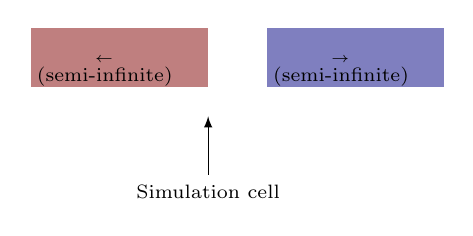
\begin{tikzpicture}[z=.5cm,>=latex,scale=.75,font=\scriptsize]
      \drawcube[draw]
      \begin{scope}[xshift=-3cm,x=3cm]
        \begin{scope}
          \drawcube[draw,densely dotted]
          \fill[red!50!black,fill opacity=0.5] (0,0,1) -- (1,0,1) -- (1,1,1) -- (0,1,1)
          -- cycle;
        \end{scope}
      \end{scope}
      \begin{scope}[xshift=1cm,x=3cm]
        \begin{scope}
          \drawcube[draw,densely dotted]
          \fill[blue!50!black,fill opacity=0.5] (0,0,1) -- (1,0,1) -- (1,1,1) -- (0,1,1)
          -- cycle;
        \end{scope}
      \end{scope}

      % Draw arrows
      \node[anchor=center,align=center] at (-1.5,.5,.5) {$\SE_\leftarrow$\\(semi-infinite)};
      \node[anchor=center,align=center] at (2.5,.5,.5) {$\SE_\rightarrow$\\(semi-infinite)};

      \draw[<-] (0.5,0,0.) -- ++(0,-1,0) node[below] {Simulation cell};
      % \draw[->] (.5,.5,.5) -- (1.5,.5,.5);
      % \draw[->] (.5,.5,.5) -- (.5,1.5,.5);

    \end{tikzpicture}

  \end{center}}

\end{frame}


\begin{frame}
  \frametitle{Electrostatic potential}
  \framesubtitle{Boundary conditions}

  \begin{block}<+->{Hartree potential}

    NEGF calculations are \emph{very} different from periodic calculations: the
    semi-infinite electrodes fix the potential at the boundaries of the device.

  \end{block}

  \begin{block}<+->{How TranSiesta imposes the bias, in 3 steps}

    \begin{enumerate}[<+->]
      \item Solve the Poisson equation via FFT\\
      $\Rightarrow$ $V_H$ is periodic and contains \emph{no} bias

      \item Add a bias correction $\delta V(\rr)$: the solution of the Laplace equation,
      $\nabla^2\delta V=0$ (no charges), with the boundary condition that the electron
      potential energy in electrode $\idxE$ is shifted by its chemical potential,
      $\delta V = \mu_\idxE$\\
      (flag: \texttt{TS.Poisson})

      \item Fix the gauge: $V_H$ is only defined up to a constant, so its average on a
      cell plane is fixed (flag: \texttt{TS.Hartree.Fix}, e.g.\ \texttt{-A})\\
      $\Rightarrow$ this sets the \emph{reference}, it does \emph{not} apply the bias

    \end{enumerate}

  \end{block}

\end{frame}


\begin{frame}
  \frametitle{Electrostatic potential}
  \framesubtitle{Choosing the bias correction $\delta V$}

  \begin{block}<+->{$N_\idxE=2$ with aligned semi-infinite directions}

    $\delta V$ is a linear ramp between the two electrodes (\texttt{TS.Poisson ramp})
    \begin{equation*}
      \delta V(x) = \mu_L + (\mu_R-\mu_L)\frac{x-x_L}{x_R-x_L},
    \end{equation*}
    with $x_{L/R}$ the positions where the left/right electrodes end.

  \end{block}

  \begin{block}<+->{Un-aligned semi-infinite directions, or $N_\idxE\neq2$}

    There is no simple analytic form for $\delta V$.

    \begin{itemize}[<+->]
      \item Default: a \emph{box} solution (\texttt{TS.Poisson elec-box}), which only sets
      $\delta V=\mu_\idxE$ inside the electrode regions and nothing in between (bad
      guess)

      \item Much better: provide an \emph{external} solution of the Laplace
      equation\footnote{\uncover<.->{This may seem like a more daunting task than it is.
            The guess is the Poisson solution \emph{without} charges, only the boundary
            conditions.}} with proper boundary conditions\\
      (\texttt{TS.Poisson V.TSV.nc})

      \item \texttt{sisl\_toolbox} creates this file: \texttt{stoolbox ts-fft} on the
      command line, or \texttt{solve\_poisson} in Python (as in TS 4)

    \end{itemize}

  \end{block}

\end{frame}


\subsection{Multi-electrode electrostatic potential}

\begin{frame}
  \frametitle{Electrostatic potential}
  \framesubtitle{Multi-electrode electrostatic potential}

  \begin{itemize}
    \item b) 6-electrode system
    \item a) Charge error $|\Delta q|$ per SCF iteration for:
    \begin{itemize}
      \item Eq.: equilibrium calculation (reference)
      \item Non-eq.\ box: default \emph{box} guess for $\delta V$
      \item Non-eq.\ MG: \emph{external} guess for $\delta V$, solved with a multigrid (MG)
      Laplace solver
    \end{itemize}
    \item<2-> Take-away: a physically correct $\delta V$ gives a better starting point for
    the SCF, i.e.\ a smaller initial $|\Delta q|$
  \end{itemize}

  \begin{center}
    \incg[width=.8\linewidth]{ts-poisson-initial}
  \end{center}

  \begin{block}<2->{Help needed!}

    This is where TranSiesta could benefit the most from external help!

    A proper, Poisson solver with arbitrary boundary conditions.

  \end{block}

\end{frame}
